\documentclass[8pt]{beamer}
\mode<presentation>
{
  \usetheme{Frankfurt}%Warsaw
  \setbeamercovered{transparent}
}
\usepackage[english]{babel}
\usepackage{graphics}
\usepackage[latin1]{inputenc}
\usepackage{times}
\usepackage[T1]{fontenc}
\usepackage{psfrag}


\title[Kalman Filtering in Video Coding] {\textbf{Kalman Filtering in Video Coding}}
\author{{\textbf{Pravin Kumar Rana\vspace{2mm}}}{\\SIP, School of Electrical Engineering\\ Kungliga Tekniska h�gskolan \\ SE-$100 44$ Stockholm}}
%\institute{(\emph{\textbf{IEEE Signal Processing Letters}, Vol. $14$, No. $9$, September $2007$})}

\begin{document}

\begin{frame}
  \titlepage
  %\begin{center}
  %\textcolor[rgb]{0.29,0.29,0.29}{\textbf{Pravin Kumar Rana}} \textcolor[rgb]{0.29,0.29,0.29}{\\SIP, School of Electrical Engineering\\ Kungliga Tekniska h�gskolan \\ SE-$100 44$ Stockholm}
  %\end{center}
\end{frame}

\begin{frame}
\begin{block}{Outline}
\begin{itemize}
  \item Introduction : Video Coding\vspace{3mm}
  \item Motion Estimation in Video Coding\vspace{3mm}
  \item Kalman Filtering Based Motion Estimation\vspace{3mm}
  \item Conclusions
\end{itemize}

\end{block}

\end{frame}


%================================================================================================================================================
%================================================================================================================================================
\section{Introduction}
\subsection[Video Coding]{Video Coding}
\begin{frame}{Video Coding}

\begin{itemize}
  \item Raw video contains an immense amount of redundant data.\vspace{1.5mm}
  \begin{center}
   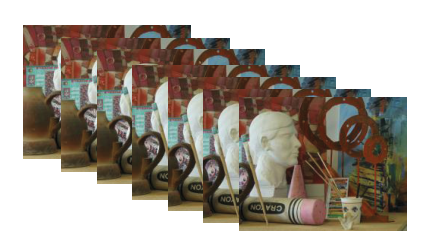
\includegraphics[width=3.5cm,angle=0]{videoframes.eps}
\end{center}
  \item Communication and storage capabilities are limited and expensive.
  \small{\begin{itemize}
    \item \textcolor[rgb]{0.00,0.00,1.00}{Example HDTV video signal:}\\\vspace{1.5mm}
     \textbf{-} 720x1280 pixels/frame, progressive scanning at 60 frames/s,\\\vspace{1.5mm}
    \begin{center}
    \textbf{$\{\frac{720x1280~pixels}{frames}\}\{\frac{60~frames}{sec}\}\{\frac{3~color}{pixels}\}\{\frac{8~bits}{color}\}=1.3~Gb/sec$}\vspace{1.5mm}
    \end{center}
    \textbf{-} 20 Mb/sec HDTV channel bandwidth requires compression by a factor of 70.\vspace{1.5mm}
  \end{itemize}}
  \item Compression is achieved by exploiting the redundancy inherent to video.\vspace{1.5mm}
  \item Predict current frame based on previously coded frames.\vspace{1.5mm}
  \item \underline{Technique}: {\textcolor[rgb]{0.98,0.00,0.00}{Motion-compensated (MC) Prediction}}\vspace{1.5mm}
  \end{itemize}

\end{frame}

\begin{frame}{Video Coding}
\begin{block}{Motion-compensated Prediction}
\begin{itemize}
\item It exploits similarity among video frames by using motion vectors.\vspace{2mm}
\item Motion vector estimation plays an important role in video coding systems with significant improvement in bit rate reduction.\vspace{2mm}
\item \textcolor[rgb]{0.00,0.00,1.00}{Example:} Standard coding structure of H.264/AVC.\vspace{2mm}
\end{itemize}
\end{block}

\begin{center}
   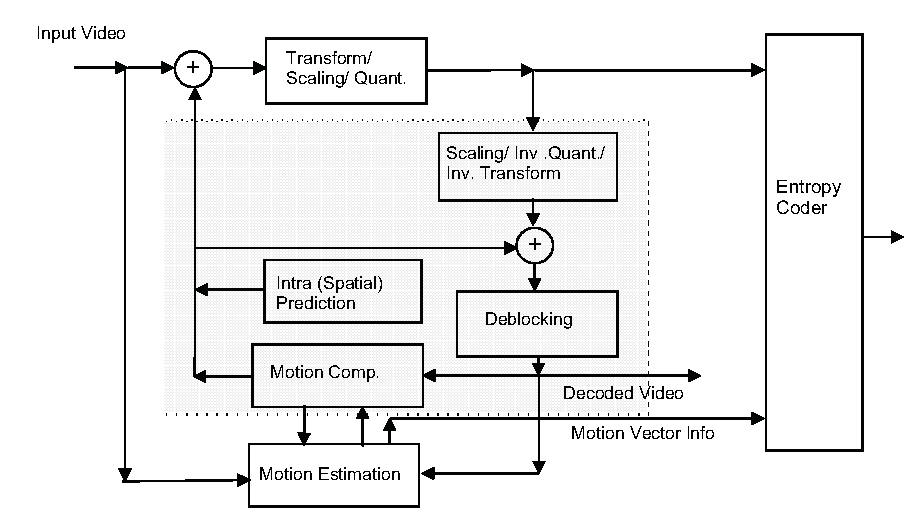
\includegraphics[width=8.5cm,angle=0]{h264_v0.eps}
\end{center}

\end{frame}

%=======================================================================================================================================
%=======================================================================================================================================

\section{Motion Estimation}
\subsection{Motion Estimation}
 \begin{frame}{Motion Estimation}
 \begin{block}{Block-Matching Algorithm}
  \begin{itemize}
   \item Divided an image frame is into non-overlapping blocks.\vspace{1.5mm}
  \begin{center}
   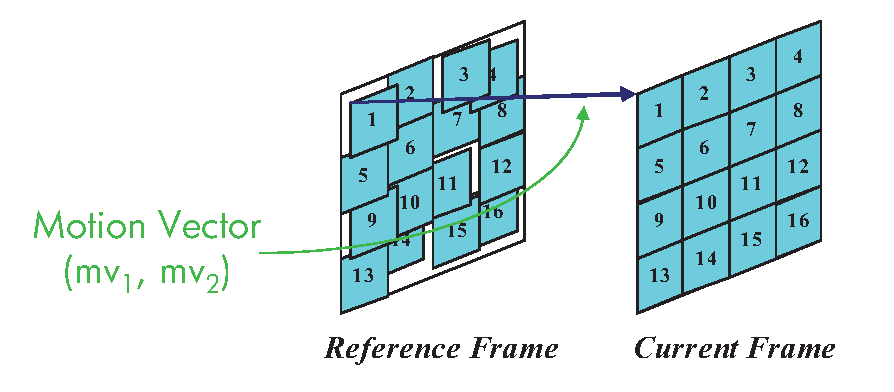
\includegraphics[width=5.5cm,angle=0]{bma.eps}
   \end{center}
   \item Motion vector of a block is estimated by searching for its best match in the previous frame.\vspace{1.5mm}
   \item \textcolor[rgb]{0.00,0.00,1}{Matching criterion}: Distortion between the current block and each searching block.\vspace{1.5mm}
   \item Resulting motion vector and a prediction error are encoded and sent to decoder.\vspace{1.5mm} 
  \end{itemize}
\end{block}
\end{frame}

\subsection{Motion Estimation}
\begin{frame}{Motion Estimation}
\psfrag{f}[c][c][0.7][0]{Previous frame}
\psfrag{g}[c][c][0.7][0]{Current frame}
\psfrag{c}[c][c][0.7][0]{Frame with motion vectors}
\psfrag{d}[c][c][0.7][0]{Without motion compensation}
\psfrag{e}[c][c][0.7][0]{After motion compensation}
\begin{center}
   \includegraphics[width=10cm,angle=0]{mv_v00.eps}
\end{center}
\end{frame}

\subsection{Motion Estimation}
\begin{frame}{Motion Estimation }
    \begin{itemize}
    \item Reduce coding rate for the prediction error\textcolor[rgb]{1,0.00,0.00}{(?)}\vspace{1.5mm}
    \item In low bit rate, motion vector bit rate is a significant part of all available budget\textcolor[rgb]{1,0.00,0.00}{(?)}\vspace{1.5mm} 
     \item Optimally allocate a limited rate budget to the motion vector and prediction error\textcolor[rgb]{1,0.00,0.00}{(?)}\vspace{1.5mm}
     \end{itemize}
\begin{block}{Rate-Distortion~(R-D) Motion Estimation}\vspace{1.5mm}
  \begin{itemize}
    \item By minimizing the following R-D cost function\vspace{1.5mm}
    \begin{center}
         $\mathnormal{J_{min}(v,\lambda)}=\sum_{\mathnormal{U^k}}\min_{\mathnormal{V}\in \mathnormal{U^k}}\{\sum_{\mathnormal{k=1}}^{\mathnormal{K}}\mathnormal{[D_{k}(\hat{v}_{k})]}+\lambda\mathnormal{R_{k}(\hat{v}_{k})}\}$\vspace{1.5mm}
    \end{center}
    \item Solution of the R-D cost function is locally optimal and globally sub-optimal.\vspace{1.5mm}
    \item It gives highly correlated smooth motion vectors.\vspace{1.5mm}
  \end{itemize}
\end{block}
\end{frame}

%=======================================================================================================================================
%=======================================================================================================================================

\section{Kalman Filtering Based Motion Estimation}
\subsection{Kalman Filtering Based Motion Estimation}
\begin{frame}{Approaches}
\begin{block}{I Kalman Filter as a Post Processing Scheme\vspace{1.5mm}}
  \begin{itemize}
    \item Extends integer-pixel accuracy of motion vectors to fractional-pixel accuracy.\vspace{2mm}
    \item Enhancing the performance of motion-compensation without increasing bit rate.\vspace{2mm}
  \end{itemize}
  \end{block}

  \begin{block}{II Kalman filter embedded R-D motion estimation\vspace{1.5mm}}
  \begin{itemize}
    \item Reduce distortion and thus lowering cost function.\vspace{2mm}
    \item Improve distortion and bit rate simultaneously.\vspace{2mm}
  \end{itemize}
  \end{block}
\end{frame}

\subsection{Kalman Filtering Based Motion Estimation}
\begin{frame}{Approach I}
\begin{block}{Kalman Filter as a Post Processing Scheme}
\begin{itemize}
  \item Measured motion vectors are obtained from the any R-D motion estimation.  \vspace{1.5mm}
  \item Generate the predicted motion vectors by utilizing the inter-block correlation.\vspace{1.5mm}
  \item Optimal estimate of motion vectors are obtain by Kalman filter. \vspace{1.5mm}
  \item State-space representation for the motion vector $[\mathnormal{v_{i, x}(m, n), v_{i, y}(m, n)}]$ of the block $(m, n)$ of the $i$-th frame,\\ \vspace{1.5mm}
  \textcolor[rgb]{0.00,0.00,1.00}{Prediction equation:}
\begin{center}
$\left[ \begin{array}{c} \upsilon_{\mathnormal{i},\mathnormal{x}}(\mathnormal{m},\mathnormal{n}) \\ \upsilon_{\mathnormal{i},\mathnormal{y}}(\mathnormal{m},\mathnormal{n}) \end{array} \right]=
\begin{bmatrix}
       \mathnormal{a_1}& 0\\[0.3em]
       0 &  \mathnormal{b_1}
     \end{bmatrix} \begin{bmatrix}
        \upsilon_{\mathnormal{i},\mathnormal{x}}(\mathnormal{m},\mathnormal{n-1})\\[0.3em]
       \upsilon_{\mathnormal{i},\mathnormal{y}}(\mathnormal{m},\mathnormal{n-1})
     \end{bmatrix}+\left[ \begin{array}{c} \mathnormal{w}_{\mathnormal{i},\mathnormal{x}}(\mathnormal{m},\mathnormal{n}) \\ \mathnormal{w}_{\mathnormal{i},\mathnormal{y}}(\mathnormal{m},\mathnormal{n})\end{array}
\right]$\end{center}

%\begin{equation}\label{1}
%    \mathbf{V}_{\mathnormal{i}}(\mathnormal{m},\mathnormal{n}) = \Phi_{\mathnormal{i}}(\mathnormal{m},\mathnormal{n-1}) \mathbf{V}_{\mathnormal{i}}(\mathnormal{m},\mathnormal{n-1})+\Gamma(\mathnormal{m},\mathnormal{n})\mathbf{w}_{\mathnormal{i}}(\mathnormal{m},\mathnormal{n})
%\end{equation}

\textcolor[rgb]{0.00,0.00,1.00}{Measurement equation:}
\begin{center}
$\left[ \begin{array}{c} \mathnormal{z}_{\mathnormal{x}}(\mathnormal{m},\mathnormal{n}) \\ \mathnormal{z}_{\mathnormal{y}}(\mathnormal{m},\mathnormal{n}) \end{array} \right]=\begin{bmatrix}
       1 & 0\\[0.3em]
       0 & 1
     \end{bmatrix} \begin{bmatrix}
        \upsilon_{\mathnormal{i},\mathnormal{x}}(\mathnormal{m},\mathnormal{n})\\[0.3em]
       \upsilon_{\mathnormal{i},\mathnormal{y}}(\mathnormal{m},\mathnormal{n})
     \end{bmatrix}+\left[ \begin{array}{c} \mathnormal{n}_{\mathnormal{x}}(\mathnormal{m},\mathnormal{n}) \\ \mathnormal{n}_{\mathnormal{y}}(\mathnormal{m},\mathnormal{n})\end{array}
\right]$\end{center}


\end{itemize}
\end{block}
\end{frame}

\subsection{Kalman Filtering Based Motion Estimation}
\begin{frame}{Approach I}
\begin{center}
   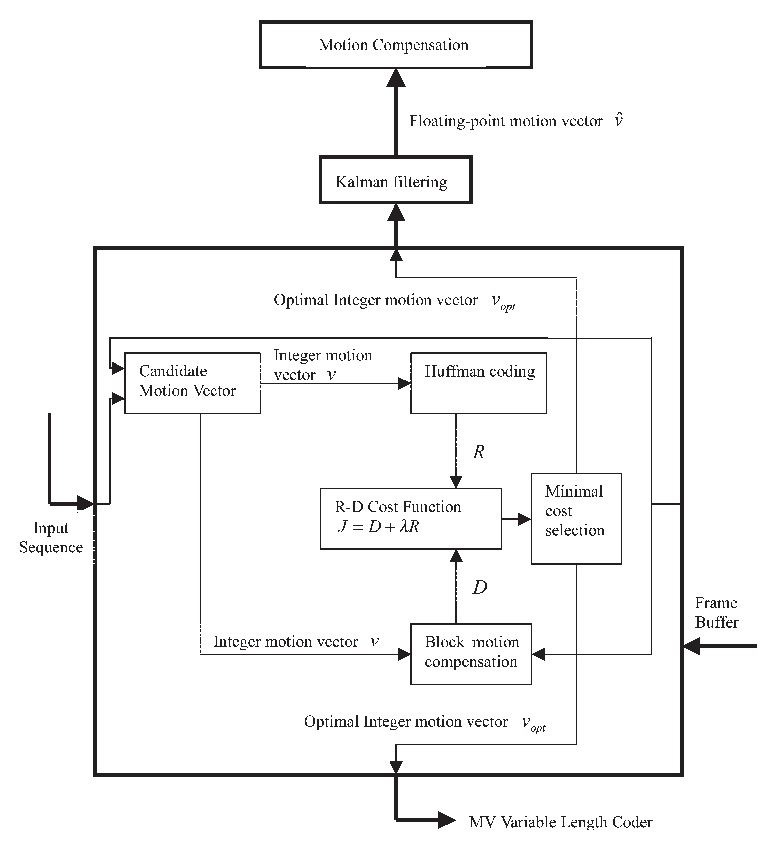
\includegraphics[width=7cm,angle=0]{kalman_v2.eps}
\end{center}
\end{frame}

\subsection{Kalman Filtering Based Motion Estimation}
\begin{frame}{Approach II}
\begin{block}{Kalman Filter Embedded Motion Estimation}
\begin{itemize}
 % \item The motion vector is not optimal from distortion viewpoint.\vspace{1.5mm}
%  \item Introduce Kalman filter into the R-D motion estimation process.\vspace{1.5mm}
  \item Obtain an optimal estimate of motion vector by using the Kalman filter\vspace{1.5mm}
  \item Cost function of Kalman filter embedded R-D motion estimation.\vspace{1.5mm}
    \begin{center}
    $\mathnormal{J_{min}(v,\lambda)}=\min_{\mathnormal{V}\in \mathnormal{U^k}}\{Kalman\mathnormal{[D_{k}(\hat{v}_{k})]}+\lambda\mathnormal{R_{k}(\hat{v}_{k})}\}$
    \end{center}
  \item $Kalman\mathnormal{[D_{k}(\hat{v}_{k})]}$ is obtain by generating prediction error using fractional-point motion vector.\vspace{1.5mm}
  \item Total cost function is reduced due to increase in compensation accuracy.\vspace{1.5mm}
\end{itemize}
\end{block}
\end{frame}

\subsection{Kalman Filtering Based Motion Estimation}
\begin{frame}{Approach II}
\begin{center}
   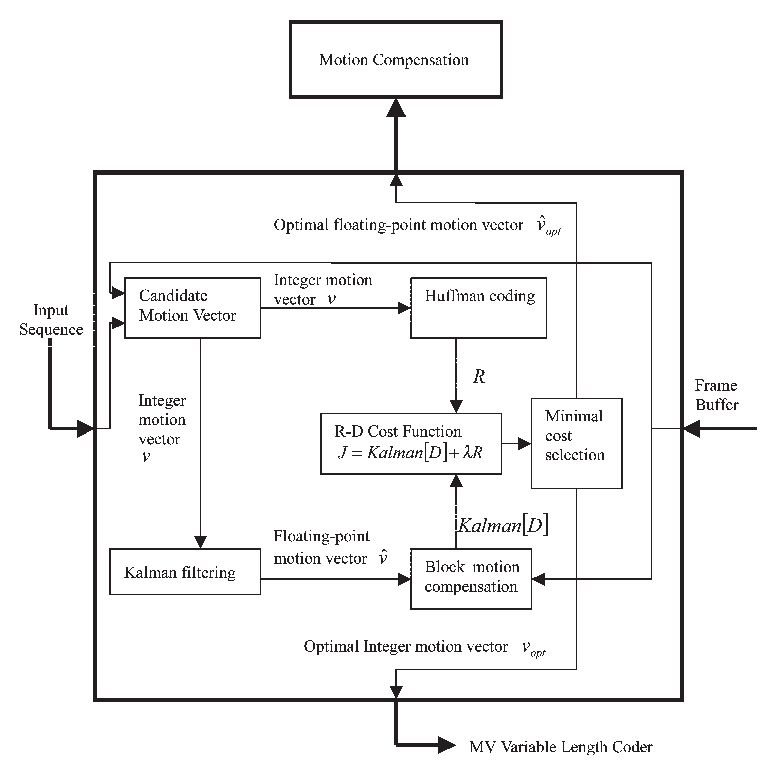
\includegraphics[width=7.5cm,angle=0]{kalman_v3.eps}
\end{center}
\end{frame}

\section{}
\begin{frame}{Conclusion}
\begin{itemize}
  \item Provide fractional-pixel accuracy motion vector at low computation complexity.\vspace{3mm}
  \item Achieves higher prediction quality without increasing the motion vectors bit rate.\vspace{3mm}
  \item Improve the rate-distortion performance.\vspace{3mm}
\end{itemize}
\end{frame}
\end{document}
